\section{L'esperimento nel mondo reale}
\label{sec:sistema-reale}
Il sistema che ho costruito è mostrato in \autoref{fig:foto-sistema}.

\begin{figure}[H]
    \centering
    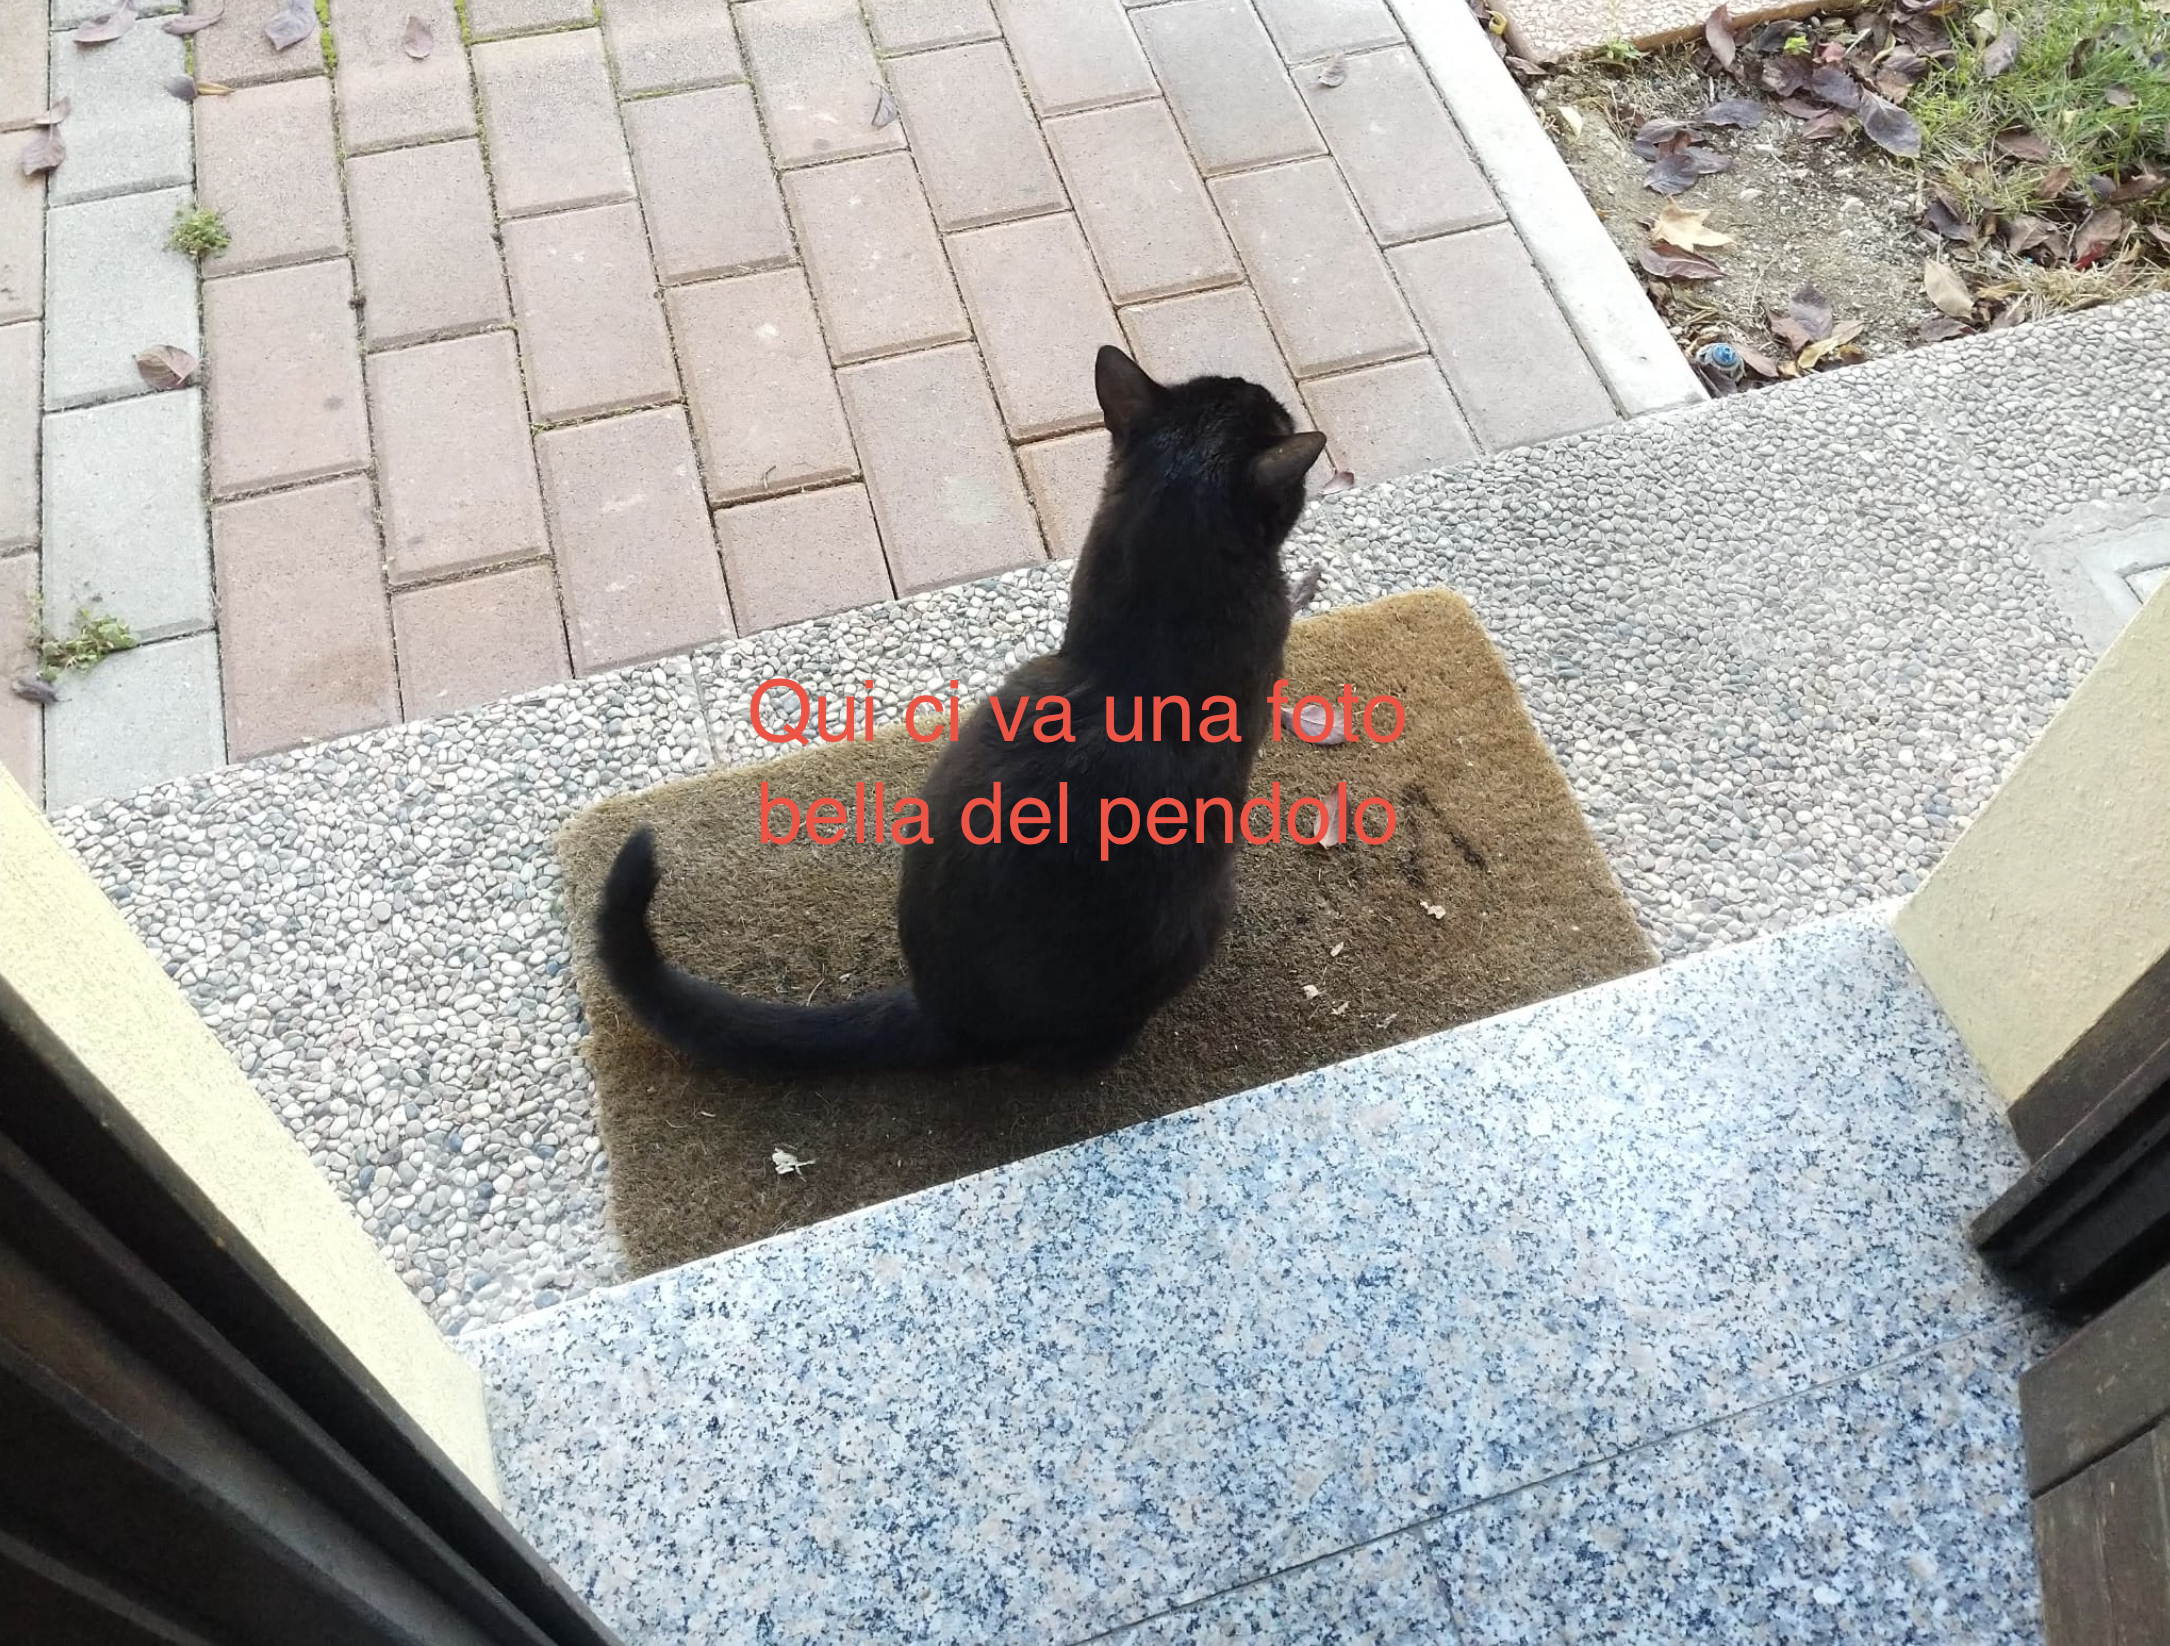
\includegraphics[width=\textwidth]{assets/foto-pendolo}
    %todo
    %todo
    \caption[Foto dell'esperimento]{aaaaaa}
    \label{fig:foto-sistema}
\end{figure}

\subsection{Componenti elettroniche}
Riporto di seguito le componenti elettroniche rilevanti del sistema.
\begin{itemize}
    \item Due encoder ottici rotativi modello \emph{LPD3806} misurano l'angolo
    del pendolo e la posizione del carrello.
    Gli encoder sono incrementali, quindi devono essere azzerati manualmente
    ogni volta che si avvia l'esperimento.

    \item Un microcontrollore \emph{ESP-32} è collegato al primo encoder.

    \item Un secondo microcontrollore \emph{ESP-32} è collegato al
    secondo encoder e al resto delle componenti.

    \item Il motore è controllato da un circuito a \emph{H-Bridge}
    modello \emph{BTS7960}.

    \item Un alimentatore da $12V$ fornisce energia al motore.

    \item Due alimentatori da $5V$ forniscono energia ai microcontrollori
    e agli encoder.
\end{itemize}

Un encoder rotativo funziona inviando un segnale elettrico ogni volta che
viene rilevata una rotazione di una frazione di angolo.
Per misurare l'angolo è quindi necessario contare il numero di impulsi
ricevuti.
I microcontrollori \emph{ESP-32} hanno un processore a \emph{due core}.
Ho scelto di usare questi così da poter usare un core in ciascuno solo per
contare gli impulsi.
L'altro core si occupa, in un caso, di inviare dati all'altro microcontrollore
e, nell'altro, di ricevere dati e di inviare il segnale di controllo al motore.

\subsection{Componenti meccaniche}
Ho usato prevalentemente componenti standard di \emph{OpenBuilds},
assieme a supporti realizzati con la stampa-3D.
Riporto di seguito le componenti meccaniche rilevanti del sistema.
\begin{itemize}
    \item La rotaia è un profilato in alluminio \emph{V-Slot} lungo $1m$.

    \item Il carrello scorre sulla rotaia, supportato da ruote \emph{Mini-V}.
    La forma delle ruote combacia con la forma del profilato, garantendo
    un movimento lineare senza vibrazioni e con basso attrito.

    \item Il carrello è collegato al motore tramite una cinghia dentata \emph{GT-2}.
    La cinghia è di gomma com un cuore di metallo, non deformabile.

    \item Il motore è un modello \emph{XD-3420} spazzolato a corrente continua
    con tensione nominale di $12V$.

    \item Due supporti ai lati della rotaia reggono il motore e il primo
    encoder rotativo.
    Motore ed encoder fungono da perni per la cinghia.

    \item Sul carrello è montato il secondo encoder rotativo,
    che funge da perno per il pendolo.

    \item Il cavo collegato al secondo encoder è lasciato pendere.
    Il suo effetto sul sistema è trascurabile.

    \item Tutto è montato su una base di legno.

\end{itemize}
